\section{Case study}
\label{sect:case-study} %
%%%%%%%%%%%%%%%%%%%%%%%%%%%%%%%%%%%%

In this section, we present a relatively complex case study, named OrderMan (Order management). The aim is to investigate how our proposed software development method is applied to develop software for a real-world problem domain. A key objective is to construct a process model of AGL from both structural and behavioral aspects that are sufficiently expressive for the domain requirements. 
\begin{figure*}[ht]
	\centering
	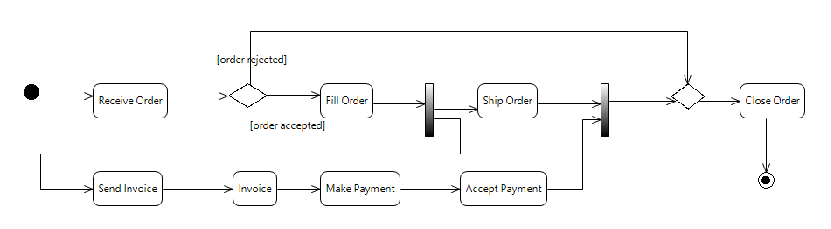
\includegraphics[scale=1.0]{case-study}
	\caption{the Process Order} %
	\label{fig:case-study}
\end{figure*}


Figure~\ref{fig:case-study} shows the UML model Process Order expresses the OrderMan’s requirements. The model consists of the five essential UML activity modeling patterns (Sequential, Decisional, Forked , Joined and Merged).


In the Figure~\ref{fig:domain-model-orderman} show the domain model of OrderMan includes the main classes (CustOrder, Shipmenet, Pament and Invoice), the association classes (Deliver, AcceptOrnot, EndOrder and CompleteOrder) and the coordinator class (FillOrder, CollectPayment, ShipOrder and AcceptPayment).
\begin{figure*}[ht]
	\centering
	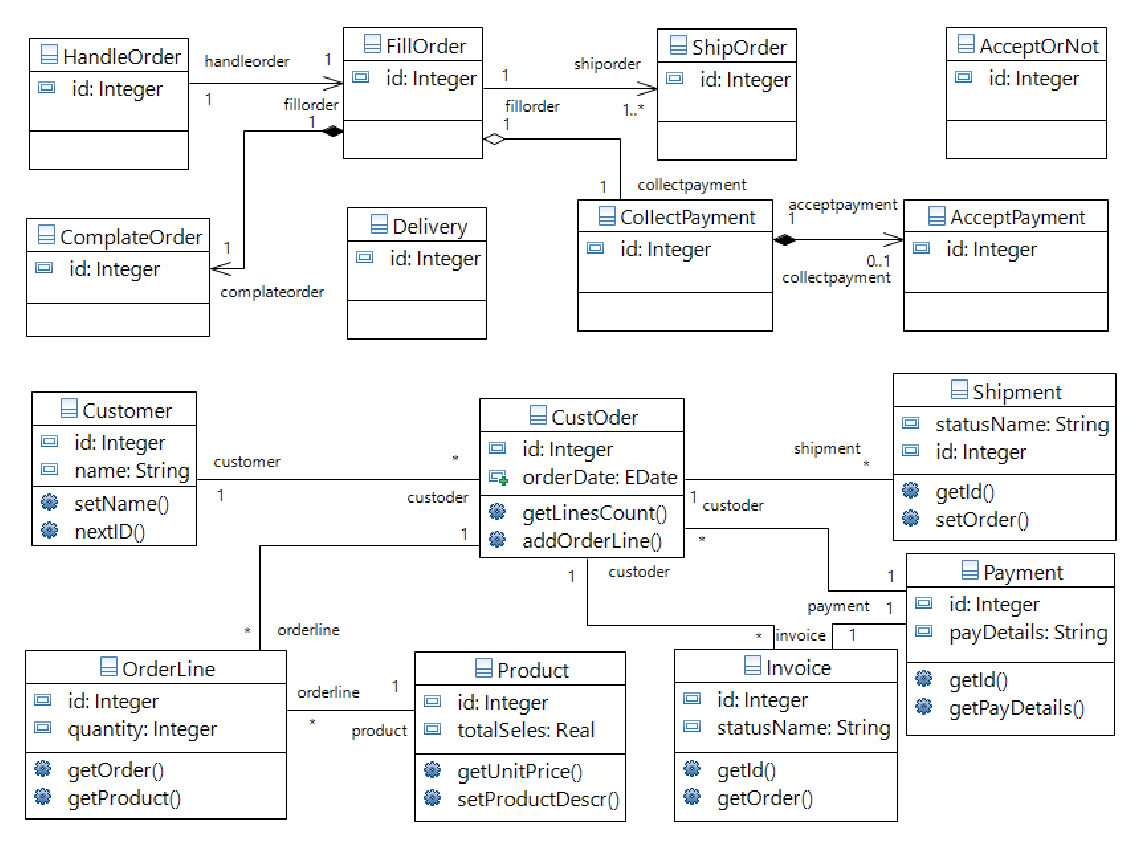
\includegraphics[scale=0.8]{domain-model-orderman}
	\caption{ The essential domain model of OrderMan} %
	\label{fig:domain-model-orderman}
\end{figure*}

In the Figure~\ref{fig:case-study-incorporate} each activity class (LHS) is attached to an activity graph that describes the behavioral logic, the developer create a set of initial unified models and associated activity graphs use Node objects, Edge objects and ModuleAct objects (RHS) to generate the software from this model.
%
\begin{figure*}[ht]
	\centering
	\includegraphics[scale=0.5]{case-study-incorporate}
	\caption{(LHS) The the unified model; (RHS) The Node objects, Edge objects of the activity graph and ModuleAct objects that are referenced by the Nodes} %
	\label{fig:case-study-incorporate}
\end{figure*}